\documentclass[11pt,compress,t,notes=noshow, aspectratio=169, xcolor=table]{beamer}

\usepackage{../../style/lmu-lecture}

% Defines macros and environments
% This file is included in slides and exercises

% Rarely used fontstyle for R packages, used only in 
% - forests/slides-forests-benchmark.tex
% - exercises/single-exercises/methods_l_1.Rnw
% - slides/cart/attic/slides_extra_trees.Rnw
\newcommand{\pkg}[1]{{\fontseries{b}\selectfont #1}}

% Spacing helpers, used often (mostly in exercises for \dlz)
\newcommand{\lz}{\vspace{0.5cm}} % vertical space (used often in slides)
\newcommand{\dlz}{\vspace{1cm}}  % double vertical space (used often in exercises, never in slides)
\newcommand{\oneliner}[1] % Oneliner for important statements, used e.g. in iml, algods
{\begin{block}{}\begin{center}\begin{Large}#1\end{Large}\end{center}\end{block}}

% Don't know if this is used or needed, remove?
% textcolor that works in mathmode
% https://tex.stackexchange.com/a/261480
% Used e.g. in forests/slides-forests-bagging.tex
% [...] \textcolor{blue}{\tfrac{1}{M}\sum^M_{m} [...]
% \makeatletter
% \renewcommand*{\@textcolor}[3]{%
%   \protect\leavevmode
%   \begingroup
%     \color#1{#2}#3%
%   \endgroup
% }
% \makeatother


\title{Interpretable Machine Learning}
% \author{LMU}
%\institute{\href{https://compstat-lmu.github.io/lecture_iml/}{compstat-lmu.github.io/lecture\_iml}}
\date{}
%\bibliography{feature-importance}

\begin{document}
    
    \newcommand{\titlefigure}{figure_man/feature-importance.png}
    \newcommand{\learninggoals}{
    	\item Understand motivation for feature importance
    	\item Develop an intuition for possible use-cases
    	\item Know characteristics of feature importance methods}
	
	% Set style/preamble.Rnw as parent.
	
	% Load all R packages and set up knitr
	
	% This file loads R packages, configures knitr options and sets preamble.Rnw as 
	% parent file
	% IF YOU MODIFY THIS, PLZ ALSO MODIFY setup.Rmd ACCORDINGLY...
	
	% Defines macros and environments

	\lecturechapter{Introduction to loss-based feature importance}
	\lecture{Interpretable Machine Learning}
	
	% ------------------------------------------------------------------------------

\begin{frame}{Motivation}
\begin{itemize}
  \item<1-3> \textbf{Feature effects} describe the relationship of features $x$ with the prediction $\yh$
  \begin{itemize}
    \item requires one plot per feature
    \item does not take the true target $y$ into account
  \end{itemize}
  \item<2-3> \textbf{Feature importance} methods quantify the relevance of features w.r.t. prediction performance
  \begin{itemize}
    \item condensed to one number per feature
    \item provides insight into the relationship with $y$
  \end{itemize}
  \item<3> \textbf{N.B.}: 
  Here, we use the term feature importance to describe loss-based feature importance methods. In the literature, you may find other notions of ``feature importance'' (e.g., variance-based methods derived from feature effect methods, see also \citebutton{Greenwell et al. (2020)}{https://doi.org/10.32614/RJ-2020-013})
\end{itemize}
\end{frame}

\begin{frame}{Example}

Feature importance offers condensed summary of feat. relevance w.r.t. performance

\medskip

\begin{itemize}
    \item Fit random forest on bike sharing data
    \item Left: Feature importance ranking by permutation feature importance (PFI)
    \item Right: Feature effects for all features
\end{itemize}

\centering
\begin{columns}[c, totalwidth=\textwidth]
  \begin{column}{0.37\textwidth}
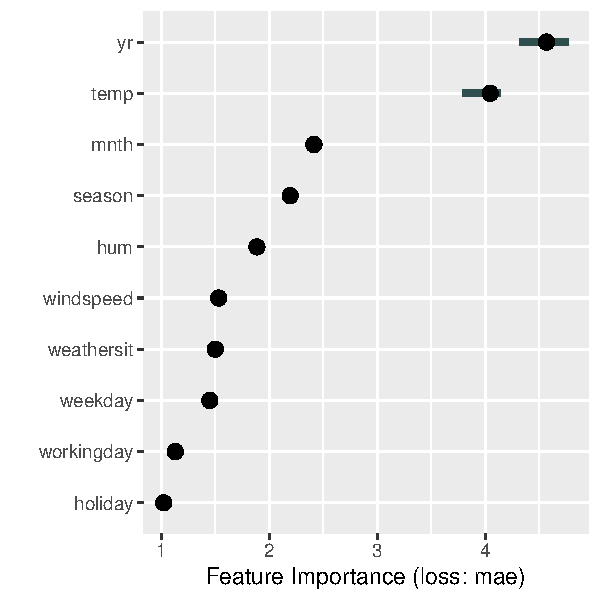
\includegraphics[width=.98\linewidth]{figure_man/bike_pfi}
\end{column}
  \begin{column}{0.63\textwidth}
  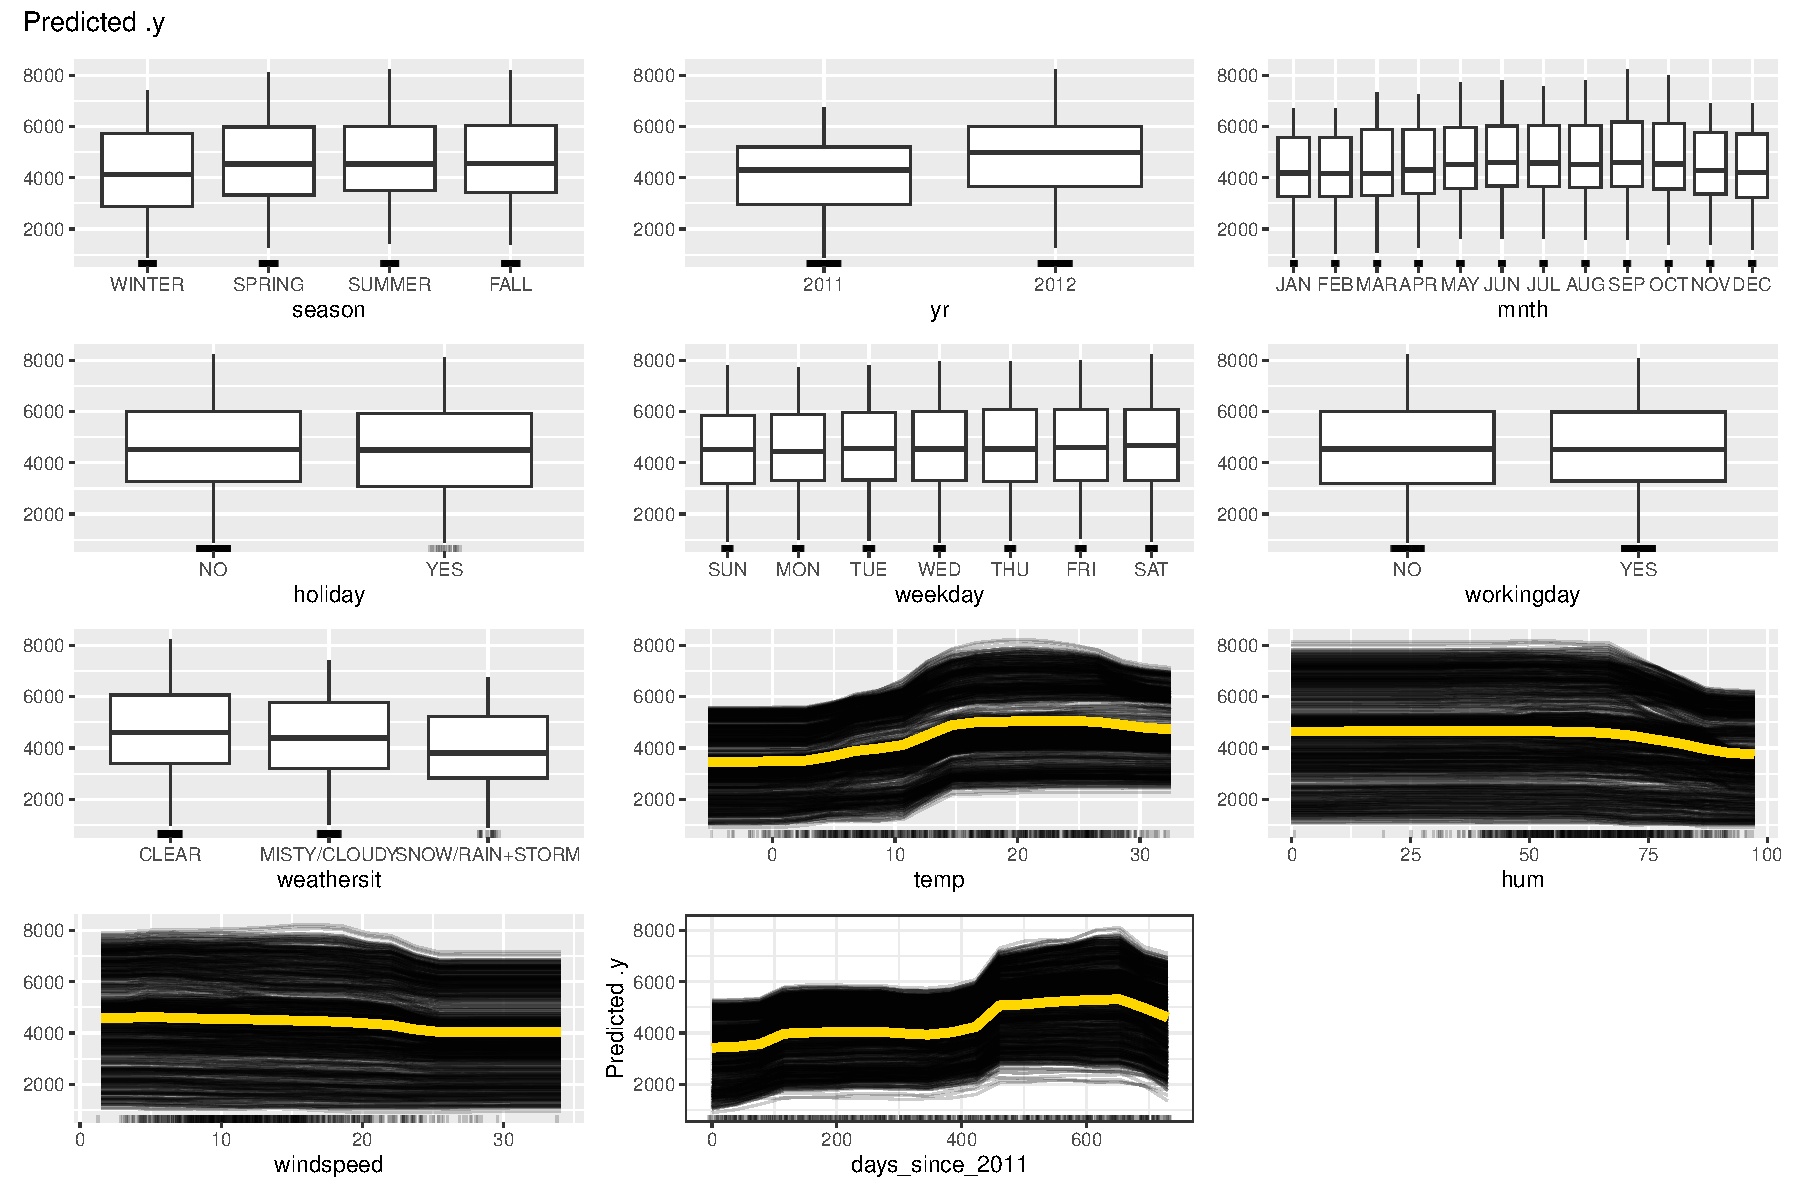
\includegraphics[width=\linewidth]{figure_man/bike_pdp+ice}
\end{column}
\end{columns}
% \begin{center}
%   \begin{figure}
%   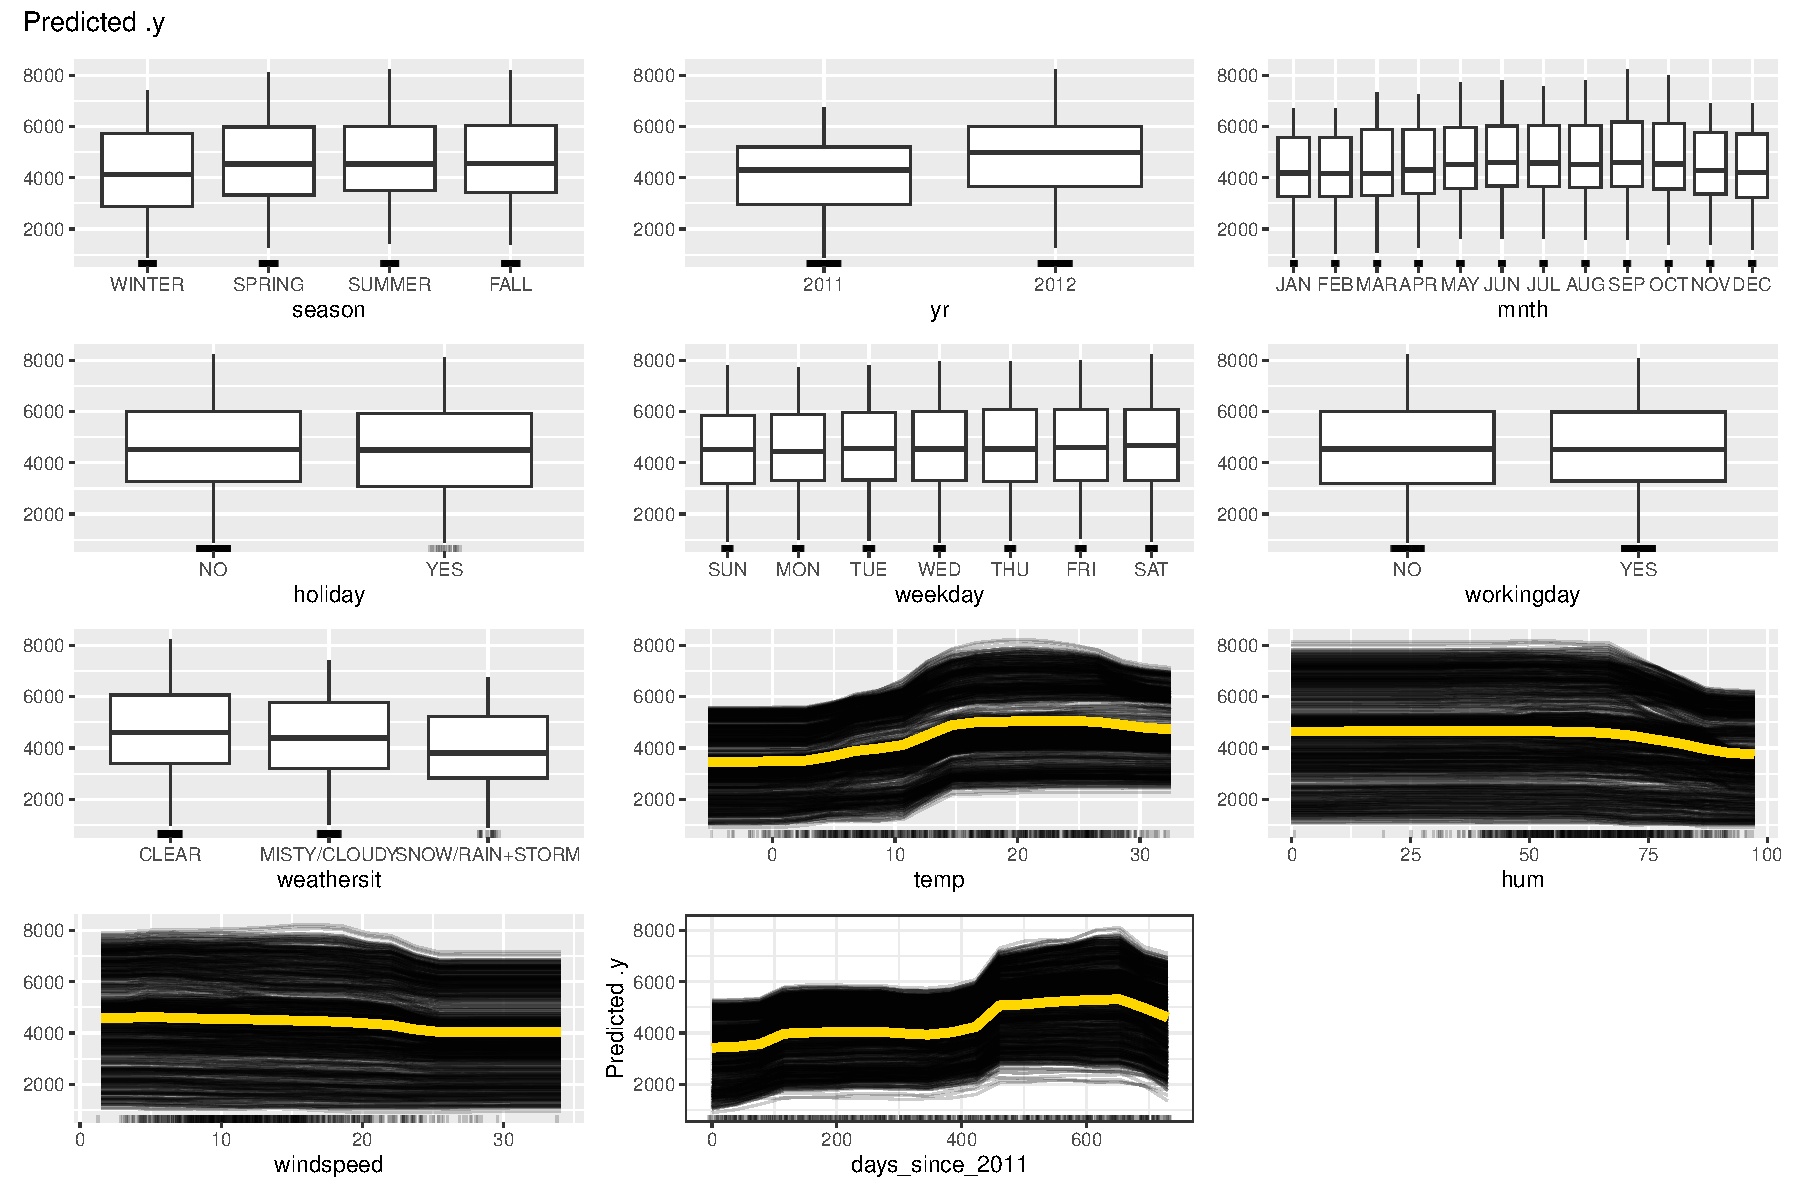
\includegraphics[width=0.55\linewidth]{figure_man/bike_pdp+ice} \hfill 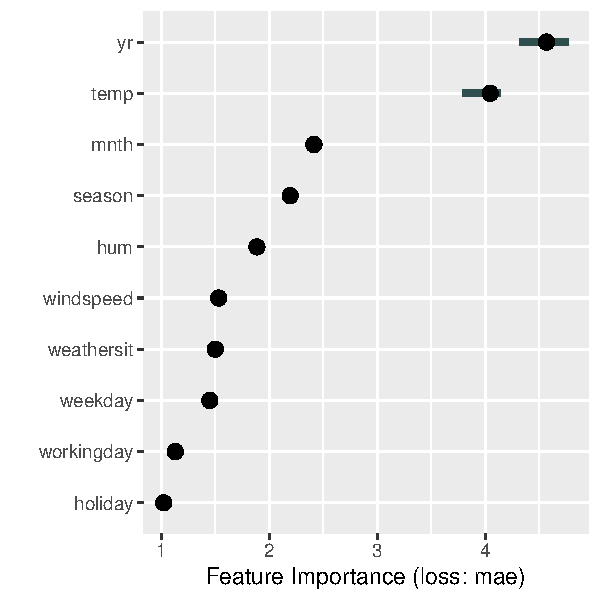
\includegraphics[width=0.35\linewidth]{figure_man/bike_pfi}
% \end{figure}
% \end{center}

\end{frame}

\begin{frame}{Feature Importance Scheme}
Loss-based feature importance methods are often based on two concepts
\lz
\begin{enumerate}
  \item \textbf{Perturbation/Removal:}\\
  Generate predictions for which the feature of interest has been perturbed or removed
  \item \textbf{Performance Comparison:} \\
  Compare performance under perturbation/removal with the original model performance
\end{enumerate}
\lz
Depending on the type of perturbation/removal, feature importance methods provide insight into different aspects of model and data.
\end{frame}


\begin{frame}{Potential Interpretation Goals}

Feature importance methods provide condensed insights, but can only highlight certain aspects of model and data. There are different interpretation goals one might be interested in whose question of interest do not necessarily coincide (except for special cases).
%Except for special cases, several questions of interest do not coincide.

\lz

For example, one may be interested in getting insight into whether the ...

\begin{enumerate}
    \item[(1)] feature $x_j$ is causal for the prediction?
    \only<2>{\begin{itemize}
      \item Changing feature value $x_j$ has an effect on prediction $\yh = \fh(x)$
      \item In LM: non-zero coefficient, in ML: present feature effect
      \item \textbf{Note:} If $x_j$ is causal for prediction $\yh$ $\nRightarrow$ causal for the ground truth $y$, e.g.:
      %A feature being causal for prediction $\yh$ does not imply that the underlying variable is causal for the ground truth $y$, e.g.:
      \begin{itemize}
          \item A disease symptom may be used in a model to predict disease status \\
          $\leadsto$ causal for prediction $\yh$
          \item But intervening on disease symptom does not have an effect on the disease \\
          $\leadsto$ not causal for the ground truth $y$
      \end{itemize}
    \end{itemize}}
    \item[(2)] feature $x_j$ contains prediction-relevant information about $y$?
    \item[(3)] model requires access to $x_j$ to achieve it's prediction performance?
\end{enumerate}
\end{frame}


\begin{frame}[c]{Example: Causal for the prediction (1)}

\begin{columns}[c, totalwidth = \textwidth]
  \begin{column}{0.6\linewidth}
    \begin{figure}
  \begin{tikzpicture}[thick, scale=1.1, every node/.style={scale=1, line width=0.25mm, black, fill=white}]
		%
		\node[draw, ellipse, scale=0.7] (x7) at (0, 2) {contacts};
		\node[draw, ellipse, scale=0.7] (x0) at (0, 1) {trust};
		\node[draw, ellipse, scale=0.7] (x1) at (0, 0) {vaccinated};
		\node[draw, ellipse, scale=0.7] (x4) at (0, -1) {test};
		%\node[draw, ellipse, scale=0.7] (x5) at (0, -2) {compliance};
		\node[draw, ellipse, scale=0.7] (y) at (-2,-.5) {$Y$: COVID risk};
		\node[draw, ellipse, scale=0.7] (x6) at (0, -2) {noise};
		\draw[dashed,gray] (-3.25,-2.5) -- (1,-2.5) -- (1,2.5) -- (-3.25,2.5) -- cycle;
		\node[scale=0.7] (dots) at (-1,-2.75) {data level};
		\draw[->] (x0) -- (x1);
		\draw[->] (x1) -- (y);
		\draw[->] (y) -- (x4);
		%\draw[->] (x5) -- (x4);
		\draw[->] (x7) -- (y);
		%\draw[-] (xd) -- (y);
		
		\node[draw, ellipse, scale=0.7] (ux7) at (2, 2) {\texttt{cnt}};
		\node[draw, ellipse, scale=0.7] (ux0) at (2, 1) {\texttt{trust}};
		\node[draw, ellipse, scale=0.7, fill=orange] (ux1) at (2, 0) {\texttt{vac}};
		\node[draw, ellipse, scale=0.7, fill=orange] (ux4) at (2, -1) {\texttt{test}};
		%\node[draw, ellipse, scale=0.7, fill=orange] (ux5) at (2,-2) {\texttt{cmpl}};
        \node[draw, ellipse, scale=0.7, fill=orange] (ux6) at (2,-2) {\texttt{noise}};
		\draw[dashed,gray] (1.25,-2.5) -- (3.5,-2.5) -- (3.5,2.5) -- (1.25,2.5) -- cycle;
		\node[scale=0.7] (dots) at (2.5,-2.75) {model level};
		\draw[->, dotted] (x1) -- (ux1);
		\draw[->, dotted] (x4) -- (ux4);
		\draw[->, dotted] (x0) -- (ux0);
		%\draw[->, dotted] (x5) -- (ux5);
		\draw[->, dotted] (x6) -- (ux6);
		\draw[->, dotted] (x7) -- (ux7);
		
		\node[draw, circle, scale=0.7] (yhat) at (3.2, -.5) {$\hat{Y}$};
		\draw[->] (ux1) -- (yhat);
		\draw[->] (ux4) -- (yhat);
		%\draw[->] (ux5) -- (yhat);
		\draw[->] (ux6) -- (yhat);
\end{tikzpicture}
\end{figure} 
  \end{column}
  \hspace{0.2cm}
  \begin{column}{0.4\linewidth}
  A feature may be causal for the prediction $\yh$ (1) without containing prediction-relevant information about $y$ (2)\\ 
  \textit{Examples:} overfitting due noisy features
  \pause
    \begin{itemize}
      \item All features used by the model are of interest
      \item Here: Model uses feature \code{noise}, although it does not contain prediction-relevant information about $y$ (data level)
      \item[$\Rightarrow$] Overfitted models may use many noise features which are deemed relevant on model level (but not on data level)
  \end{itemize}
  \end{column}
\end{columns}

\end{frame}


\begin{frame}{Potential Interpretation Goals}

Feature importance methods provide condensed insights, but can only highlight certain aspects of model and data. There are different interpretation goals one might be interested in whose question of interest do not necessarily coincide (except for special cases).
%Except for special cases, several questions of interest do not coincide.

\lz

For example, one may be interested in getting insight into whether the ...

\begin{enumerate}
    \item[(1)] feature $x_j$ is causal for the prediction?
    \item[(2)] feature $x_j$ contains prediction-relevant information about $y$?
    \begin{itemize}
      \item Feature $x_j$ helps to predict the target $y$ (e.g., conditional expectation) w.r.t. performance 
      %, as measured by the difference in expected loss
      %%\item e.g. when $\E[y|x_j] \neq \E[y]$ for models that minimize MSE
      %\item feature selection terminology: \textit{weak relevance} \citebutton{Pellet (2008)}{https://www.jmlr.org/papers/volume9/pellet08a/pellet08a.pdf}
      \item If $x_j \indep y$ (independent) then $x_j$ and $y$ have zero mutual information (since $\E[y|x_j] = \E[y]$)\\ %and therefore cannot contain 
      $\leadsto$ $x_j$ has no prediction-relevant information
    \end{itemize}
    \item[(3)] model requires access to $x_j$ to achieve it's prediction performance?
\end{enumerate}
\end{frame}




\begin{frame}[c]{Example: Contains prediction-relevant information (2)}

\begin{columns}[c, totalwidth=\textwidth]
  \begin{column}{0.6\textwidth}
  \begin{figure}
  \begin{tikzpicture}[thick, scale=1.1, every node/.style={scale=1, line width=0.25mm, black, fill=white}]
		%
		\node[draw, ellipse, scale=0.7, fill=orange] (x7) at (0, 2) {contacts};
		\node[draw, ellipse, scale=0.7, fill=orange] (x0) at (0, 1) {trust};
		\node[draw, ellipse, scale=0.7, fill=orange] (x1) at (0, 0) {vaccinated};
		\node[draw, ellipse, scale=0.7, fill=orange] (x4) at (0, -1) {test};
		%\node[draw, ellipse, scale=0.7] (x5) at (0, -2) {compliance};
		\node[draw, ellipse, scale=0.7] (y) at (-2,-.5) {$Y$: COVID risk};
		\node[draw, ellipse, scale=0.7] (x6) at (0, -2) {noise};
		\draw[dashed,gray] (-3.25,-2.5) -- (1,-2.5) -- (1,2.5) -- (-3.25,2.5) -- cycle;
		\node[scale=0.7] (dots) at (-1,-2.75) {data level};
		\draw[->] (x0) -- (x1);
		\draw[->] (x1) -- (y);
		\draw[->] (y) -- (x4);
		%\draw[->] (x5) -- (x4);
		\draw[->] (x7) -- (y);
		%\draw[-] (xd) -- (y);
		
		\node[draw, ellipse, scale=0.7] (ux7) at (2, 2) {\texttt{cnt}};
		\node[draw, ellipse, scale=0.7] (ux0) at (2, 1) {\texttt{trust}};
		\node[draw, ellipse, scale=0.7] (ux1) at (2, 0) {\texttt{vac}};
		\node[draw, ellipse, scale=0.7] (ux4) at (2, -1) {\texttt{test}};
		%\node[draw, ellipse, scale=0.7] (ux5) at (2,-2) {\texttt{cmpl}};
        \node[draw, ellipse, scale=0.7] (ux6) at (2,-2) {\texttt{noise}};
		\draw[dashed,gray] (1.25,-2.5) -- (3.5,-2.5) -- (3.5,2.5) -- (1.25,2.5) -- cycle;
		\node[scale=0.7] (dots) at (2.5,-2.75) {model level};
		\draw[->, dotted] (x1) -- (ux1);
		\draw[->, dotted] (x4) -- (ux4);
		\draw[->, dotted] (x0) -- (ux0);
		%\draw[->, dotted] (x5) -- (ux5);
		\draw[->, dotted] (x6) -- (ux6);
		\draw[->, dotted] (x7) -- (ux7);
		
		\node[draw, circle, scale=0.7] (yhat) at (3.2, -.5) {$\hat{Y}$};
		\draw[->] (ux1) -- (yhat);
		\draw[->] (ux4) -- (yhat);
		%\draw[->] (ux5) -- (yhat);
		\draw[->] (ux6) -- (yhat);
\end{tikzpicture}
\end{figure} 
  \end{column}
  \hspace{0.2cm}
  \begin{column}{0.4\textwidth}
  A feature may contain prediction-relevant information (2) without causing the prediction (1)\\ 
  \textit{Examples:} underfitting, model multiplicity
  \lz
  \pause
      \begin{itemize}
      \item All prediction-relevant features for $y$ are of interest
      \item Example: All features that are directly or indirectly (i.e., via another feature) connected to $y$ 
      \item[$\Rightarrow$] Underfitted models may ignore prediction-relevant features such as \code{contacts} here
  \end{itemize}
  \end{column}
\end{columns}
\end{frame}

\begin{frame}{Potential Interpretation Goals}

Feature importance methods provide condensed insights, but can only highlight certain aspects of model and data. There are different interpretation goals one might be interested in whose question of interest do not necessarily coincide (except for special cases).
%Except for special cases, several questions of interest do not coincide.

\lz

For example, one may be interested in getting insight into whether the ...

\begin{enumerate}
    \item[(1)] feature $x_j$ is causal for the prediction?
    \item[(2)] feature $x_j$ contains prediction-relevant information about $y$?
    \item[(3)] model requires access to $x_j$ to achieve it's prediction performance?
    \begin{itemize}
      \item Feature $x_{j}$ helps to predict the target $y$ w.r.t. performance, compared to using only $x_{-j}$  %, as measured by the difference in expected loss
      %%\item e.g. when $\E[y|x_{-j}] \neq \E[y|x_j, x_{-j}]$ for models that minimize MSE
      %\item feature selection terminology: \textit{strong relevance} \citebutton{Pellet (2008)}{https://www.jmlr.org/papers/volume9/pellet08a/pellet08a.pdf}
      \item If $x_j \indep y | x_{-j}$ (independent) then $\E[y|x_{-j}] = \E[y|x_j, x_{-j}]$ \\
      $\leadsto$ $x_j$ does not contribute unique prediction-relevant information about $y$
      \item \textbf{Note:} A model may rely on features that can be replaced with others, e.g., a random forest fitted on data with $\E[y|x_1] \neq \E[y]$ and $\E[y|x_1] = \E[y|x_1, x_2]$ where $x_1$ was not used as split variable may rely on $x_2$ %was not sampled as potential split variable may rely on $x_2$.
    \end{itemize}
\end{enumerate}
\end{frame}


\begin{frame}[c]{Example: Unique prediction relevant information (3)}


\begin{columns}[c, totalwidth=\textwidth]
  \begin{column}{0.6\textwidth}
  \begin{figure}
  \begin{tikzpicture}[thick, scale=1.1, every node/.style={scale=1, line width=0.25mm, black, fill=white}]
		%
		\node[draw, ellipse, scale=0.7, fill=orange] (x7) at (0, 2) {contacts};
		\node[draw, ellipse, scale=0.7] (x0) at (0, 1) {trust};
		\node[draw, ellipse, scale=0.7, fill=orange] (x1) at (0, 0) {vaccinated};
		\node[draw, ellipse, scale=0.7, fill=orange] (x4) at (0, -1) {test};
		%\node[draw, ellipse, scale=0.7, fill=orange] (x5) at (0, -2) {compliance};
		\node[draw, ellipse, scale=0.7] (y) at (-2,-.5) {$Y$: COVID risk};
		\node[draw, ellipse, scale=0.7] (x6) at (0, -2) {noise};
		\draw[dashed,gray] (-3.25,-2.5) -- (1,-2.5) -- (1,2.5) -- (-3.25,2.5) -- cycle;
		\node[scale=0.7] (dots) at (-1,-2.75) {data level};
		\draw[->] (x0) -- (x1);
		\draw[->] (x1) -- (y);
		\draw[->] (y) -- (x4);
		%\draw[->] (x5) -- (x4);
		\draw[->] (x7) -- (y);
		%\draw[-] (xd) -- (y);
		
		\node[draw, ellipse, scale=0.7] (ux7) at (2, 2) {\texttt{cnt}};
		\node[draw, ellipse, scale=0.7] (ux0) at (2, 1) {\texttt{trust}};
		\node[draw, ellipse, scale=0.7] (ux1) at (2, 0) {\texttt{vac}};
		\node[draw, ellipse, scale=0.7] (ux4) at (2, -1) {\texttt{test}};
		%\node[draw, ellipse, scale=0.7] (ux5) at (2,-2) {\texttt{cmpl}};
        \node[draw, ellipse, scale=0.7] (ux6) at (2,-2) {\texttt{noise}};
		\draw[dashed,gray] (1.25,-2.5) -- (3.5,-2.5) -- (3.5,2.5) -- (1.25,2.5) -- cycle;
		\node[scale=0.7] (dots) at (2.5,-2.75) {model level};
		\draw[->, dotted] (x1) -- (ux1);
		\draw[->, dotted] (x4) -- (ux4);
		\draw[->, dotted] (x0) -- (ux0);
		%\draw[->, dotted] (x5) -- (ux5);
		\draw[->, dotted] (x6) -- (ux6);
		\draw[->, dotted] (x7) -- (ux7);
		
		\node[draw, circle, scale=0.7] (yhat) at (3.2, -.5) {$\hat{Y}$};
		\draw[->] (ux1) -- (yhat);
		\draw[->] (ux4) -- (yhat);
		%\draw[->] (ux5) -- (yhat);
		\draw[->] (ux6) -- (yhat);
\end{tikzpicture}
\end{figure} 
  \end{column}
  \hspace{0.2cm}
  \begin{column}{0.4\textwidth}
  A feature may contain prediction-relevant information (2), without the model requiring access to the feature for (optimal) prediction performance (3)
   \\
   \textit{Examples:} correlated features, confounding
  
  \lz\pause
      \begin{itemize}
      \item All unique prediction-relevant features for $y$ are of interest
      \item Example: All features that are directly connected to $y$
      \item[$\Rightarrow$] \code{trust} and \code{vaccinated} may be correlated but only \code{vaccinated} is directly connected to $y$
  \end{itemize}
  \end{column}
\end{columns}  
\end{frame}

% \begin{frame}{Potential Interpretation Goals}

% Feature importance methods provide condensed insights, but can only highlight certain aspects of model and data. There are different interpretation goals one might be interested in whose question of interest do not necessarily coincide (except for special cases).
% %Except for special cases, several questions of interest do not coincide.

% \lz

% For example, one may be interested in getting insight into whether the ...

% \begin{enumerate}
% %<1|only@1>
%     \item[(1)]<1|only@1> feature $x_j$ is causal for the prediction?
%     \begin{itemize}
%       \item Changing feature value $x_j$ has an effect on prediction $\yh = \fh(x)$
%       \item In LM: non-zero coefficient, in ML: present feature effect
%       \item \textbf{Note:} 
%       A feature being causal for prediction $\yh$ does not imply that the underlying variable is causal for the ground truth $y$, e.g.:
%       \begin{itemize}
%           \item A disease symptom may be used in a model to predict disease status \\
%           $\leadsto$ causal for prediction $\yh$
%           \item But intervening on disease symptom does not have an effect on the disease \\
%           $\leadsto$ not causal for the ground truth $y$
%       \end{itemize}
%     \end{itemize}
%     \item[(2)]<2|only@2> feature $x_j$ contains prediction-relevant information about $y$?
%     \begin{itemize}
%       \item Feature $x_j$ helps to predict the target $y$ (e.g., conditional expectation) w.r.t. performance 
%       %, as measured by the difference in expected loss
%       \item e.g. when $\E[y|x_j] \neq \E[y]$ for models that minimize MSE
%       %\item feature selection terminology: \textit{weak relevance} \citebutton{Pellet (2008)}{https://www.jmlr.org/papers/volume9/pellet08a/pellet08a.pdf}
%       \item If $x_j \indep y$ (independent) then $x_j$ and $y$ have zero mutual information (since $\E[y|x_j] = \E[y]$)\\ %and therefore cannot contain 
%       $\leadsto$ $x_j$ has no prediction-relevant information
%     \end{itemize}
%     \item[(3)]<3-4|only@3-4> model requires access to $x_j$ to achieve it's prediction performance?
%     \begin{itemize}
%       \item Feature $x_{j}$ helps to predict the target $y$, compared to using only $x_{-j}$ w.r.t. performance %, as measured by the difference in expected loss
%       \item e.g. when $\E[y|x_{-j}] \neq \E[y|x_j, x_{-j}]$ for models that minimize MSE
%       %\item feature selection terminology: \textit{strong relevance} \citebutton{Pellet (2008)}{https://www.jmlr.org/papers/volume9/pellet08a/pellet08a.pdf}
%       \item If $x_j \indep y | x_{-j}$ (independent) then $\E[y|x_{-j}] = \E[y|x_j, x_{-j}]$ \\
%       $\leadsto$ $x_j$ does not contribute unique prediction-relevant information about $y$
%       \item \textbf{Note:} A model may rely on features that can be replaced with others, e.g., a random forest fitted on data with $\E[y|x_1] \neq \E[y]$ and $\E[y|x_1] = \E[y|x_1, x_2]$ where $x_1$ was not used as split variable may rely on $x_2$ %was not sampled as potential split variable may rely on $x_2$.
%     \end{itemize}
% \end{enumerate}
% \lz
% \only<4>{The distinctness of the aforementioned aspects can be proven by example (sketch).}
% \end{frame}

% \begin{frame}{Potential Interpretation Goals}

% The distinctness of the aforementioned aspects can be proven by example (sketch):

% \begin{itemize}
%   \item A feature may be causal for the prediction $\yh$ (1) without containing prediction-relevant information about $y$ (2)\\
%   \textit{Example:} overfitting
%   \item A feature may contain prediction-relevant information (2) without causing the prediction (1)\\ \textit{Examples:} underfitting, model multiplicity
%   \item A feature may contain prediction-relevant information (2), without the model requiring access to the feature for (optimal) prediction performance (3)\\
%   \textit{Note:} A model may rely on features that can be replaced with others, e.g., a random forest fitted on data with $\E[y|x_1] \neq \E[y]$ and $\E[y|x_1] = \E[y|x_1, x_2]$ where $x_1$ was not used as split variable may rely on $x_2$ %was not sampled as potential split variable may rely on $x_2$.
%   \\
%   \textit{Examples:} correlated features, confounding
%   \end{itemize}
% $\Rightarrow$ In general, an importance score cannot provide insight into all aspects at once.
% \end{frame}



% \begin{frame} {Causal for the prediction (1)}
%   \begin{figure}
%   \begin{tikzpicture}[thick, scale=1.1, every node/.style={scale=1, line width=0.25mm, black, fill=white}]
% 		%
% 		\node[draw, ellipse, scale=0.7] (x7) at (0, 2) {contacts};
% 		\node[draw, ellipse, scale=0.7] (x0) at (0, 1) {trust};
% 		\node[draw, ellipse, scale=0.7] (x1) at (0, 0) {vaccinated};
% 		%\node[draw, ellipse, scale=0.7] (x4) at (0, -1) {test};
% 		%\node[draw, ellipse, scale=0.7] (x5) at (0, -2) {compliance};
% 		\node[draw, ellipse, scale=0.7] (y) at (-2,-.5) {$Y$: COVID risk};
% 		\node[draw, ellipse, scale=0.7] (x6) at (0, -3) {noise};
% 		\draw[dashed,gray] (-3.25,-3.5) -- (1,-3.5) -- (1,2.5) -- (-3.25,2.5) -- cycle;
% 		\node[scale=0.7] (dots) at (-1,-3.75) {data level};
% 		\draw[->] (x0) -- (x1);
% 		\draw[->] (x1) -- (y);
% 		%\draw[->] (y) -- (x4);
% 		%\draw[->] (x5) -- (x4);
% 		\draw[->] (x7) -- (y);
% 		%\draw[-] (xd) -- (y);
		
% 		\node[draw, ellipse, scale=0.7] (ux7) at (2, 2) {\texttt{cnt}};
% 		\node[draw, ellipse, scale=0.7] (ux0) at (2, 1) {\texttt{trust}};
% 		\node[draw, ellipse, scale=0.7, fill=orange] (ux1) at (2, 0) {\texttt{vac}};
% 		%\node[draw, ellipse, scale=0.7, fill=orange] (ux4) at (2, -1) {\texttt{test}};
% 		%\node[draw, ellipse, scale=0.7, fill=orange] (ux5) at (2,-2) {\texttt{cmpl}};
%         \node[draw, ellipse, scale=0.7, fill=orange] (ux6) at (2,-3) {\texttt{noise}};
% 		\draw[dashed,gray] (1.25,-3.5) -- (3.5,-3.5) -- (3.5,2.5) -- (1.25,2.5) -- cycle;
% 		\node[scale=0.7] (dots) at (2.5,-3.75) {model level};
% 		\draw[->, dotted] (x1) -- (ux1);
% 		%\draw[->, dotted] (x4) -- (ux4);
% 		\draw[->, dotted] (x0) -- (ux0);
% 		%\draw[->, dotted] (x5) -- (ux5);
% 		\draw[->, dotted] (x6) -- (ux6);
% 		\draw[->, dotted] (x7) -- (ux7);
		
% 		\node[draw, circle, scale=0.7] (yhat) at (3.2, -.5) {$\hat{Y}$};
% 		\draw[->] (ux1) -- (yhat);
% 		%\draw[->] (ux4) -- (yhat);
% 		%\draw[->] (ux5) -- (yhat);
% 		\draw[->] (ux6) -- (yhat);
% \end{tikzpicture}
% \end{figure} 
% \end{frame}

\endlecture
\end{document}
